% ============================================================
%  StructRAG — main.tex
%
%  STATUS: PRE-SUBMISSION DRAFT
%  Open items before any submission:
%  (1) [AUTHOR-EMAIL] — fill real email addresses
%  (2) [FIG-ARCH]     — replace figure stub with actual diagram
%  (3) [RESCORE]      — run one pinned context-aware RAGAS judge
%                       for all 4 models; replace Table I numbers
%  (4) [FLAT-EVAL]    — run flat-baseline pipeline end-to-end
%                       through the 49-question benchmark;
%                       add column to Table I
% ============================================================
\documentclass[conference]{IEEEtran}

\usepackage{amsmath}
\usepackage{amssymb}
\usepackage{graphicx}
\usepackage{booktabs}
\usepackage[hidelinks]{hyperref}
\usepackage{cite}
\usepackage{algorithm}
\usepackage{algorithmic}
\usepackage{url}
\usepackage{tikz}
\usetikzlibrary{arrows.meta, positioning, shapes.geometric}

% ── Title ───────────────────────────────────────────────────
\title{StructRAG: Hierarchy-Aware Retrieval-Augmented Generation
for Normative Concrete Design Standards}

% ── Authors ─────────────────────────────────────────────────
\author{%
  \IEEEauthorblockN{Mohamed Khelil, Manef Belkadhi, Rached Hadj Amor}
  \IEEEauthorblockA{ESPRIT School of Engineering, Tunisia\\
    Supervisor: Afif Beji, Eng., M.Sc.\\
    % [AUTHOR-EMAIL]: replace with actual addresses
    \{khelil, belkadhi, hadjamor\}@esprit.tn}
}

\begin{document}
\maketitle

% ── Abstract ─────────────────────────────────────────────────
\begin{abstract}
Large language models are increasingly applied to technical standards
retrieval in safety-critical domains such as structural engineering.
Standard Retrieval-Augmented Generation (RAG) pipelines split documents
into fixed-size token windows, discarding the clause hierarchy that
governs how information must be read in normative codes.
Applied to Eurocode~2 (NF~EN~1992-1-1:2004), this causes
applicability conditions to be separated from the formulas that depend
on them, and national annex notes to be detached from the clauses they
modify.
This paper presents \textbf{StructRAG}, a RAG system that treats the
document's own clause structure as the primary indexing unit.
A font-metric parser produces 2{,}132 typed nodes; a hierarchy-aware
chunker assembles 467 chunks in which each chunk is one complete clause
with its full ancestor breadcrumb prepended; hybrid BM25+vector
Reciprocal Rank Fusion (RRF) retrieval and cross-encoder reranking
are layered on top, augmented by domain-specific table and formula
injectors.
Evaluated on a 49-question French/English benchmark across four large
language models, the system achieves a verified near-zero hallucination
rate on clause citations (0/44 for three of four models), answer
relevancy of 0.64--0.70, and a context recall of 0.27--0.63 depending
on model.
A 14-question ablation shows that adding BM25+RRF and table injection
raises correct-answer rate from 3/14 to 7/14; adding cross-encoder
reranking raises it further to 9/14.
The system is deployed as a Flask web application for interactive
querying of the French Eurocode~2 edition.
\end{abstract}

\begin{IEEEkeywords}
Retrieval-Augmented Generation, Eurocode~2, hierarchical chunking,
hybrid retrieval, BM25, cross-encoder reranking, hallucination
detection, RAGAS, structural engineering
\end{IEEEkeywords}

% ── 1. Introduction ──────────────────────────────────────────
\section{Introduction}
\label{sec:intro}

Structural engineers routinely consult normative codes to verify design
decisions: minimum concrete cover, partial safety factors, shear
resistance formulas, and detailing rules.
Eurocode~2 (EN~1992-1-1), the European standard for reinforced concrete
design, is a 211-page document organized into a strict hierarchy of
sections, clauses, sub-clauses, paragraphs, notes, and tables.
Mis-reading or mis-retrieving a clause can have direct structural safety
consequences.

The standard approach to LLM-assisted document
retrieval---Retrieval-Augmented Generation (RAG)~\cite{lewis2020rag}---
indexes a corpus by splitting it into fixed-length token windows.
Applied to Eurocode~2, this causes three recurring failures: a clause is
retrieved without the applicability condition it depends on; a formula
arrives without the variable definitions that constrain it; and a
national annex NOTE, which may override a recommended value, ends up
in a different chunk than the clause it modifies.

\textbf{StructRAG} addresses this by mapping the document's own
structural units directly onto retrievable chunks.
This paper makes three concrete contributions:
\begin{itemize}
  \item A font-metric structural parser for the French Eurocode~2 PDF
        producing 2{,}132 typed nodes with full ancestor breadcrumbs
        and automatic cross-reference extraction.
  \item A hierarchy-aware chunker that assembles one chunk per complete
        clause, prepending the full ancestor path to the chunk text so
        that the embedding model encodes structural provenance.
  \item A layered retrieval pipeline combining hybrid BM25+vector
        RRF~\cite{cormack2009rrf}, cross-encoder
        reranking~\cite{nogueira2019passage}, direct table injection,
        and a hand-transcribed formula library for image-rendered
        formulas.
\end{itemize}

The evaluation uses the RAGAS framework~\cite{es2023ragas} augmented by
a deterministic hallucination check that verifies every cited clause
number against the parsed node corpus---a check that is both cheap to
compute and directly interpretable for a safety-critical application.

% ── 2. Related Work ───────────────────────────────────────────
\section{Related Work}
\label{sec:related}

\subsection{Retrieval-Augmented Generation}

Lewis et al.~\cite{lewis2020rag} introduced RAG as a framework for
grounding LLM generation in non-parametric retrieval.
A survey by Gao et al.~\cite{gao2023survey} distinguishes three
generations: naive (fixed chunking, vector search), advanced (hybrid
retrieval, reranking, query rewriting), and modular (adaptive
composition).
StructRAG is an advanced RAG system with domain-specific extensions.

\subsection{Chunking Strategies}

Fixed-size sliding-window chunking is the dominant baseline.
Parent-child (small-to-big) retrieval~\cite{gao2023survey} retrieves
on fine-grained child chunks but generates from larger parent chunks.
Structure-aware chunking for regulatory documents is an active
2024--2025 direction~\cite{wang2024financial}: mapping document
structure onto chunk boundaries consistently outperforms fixed windows
on complex regulatory text.
StructRAG applies this to Eurocode~2 by using the standard's own
clause hierarchy as the chunk boundary, without choosing arbitrary
token counts.

\subsection{Hybrid Retrieval and Reranking}

BM25~\cite{robertson2009bm25} captures exact symbolic queries---Greek
symbols, clause identifiers, numeric constants---that dense embeddings
tend to mishandle.
Reciprocal Rank Fusion~\cite{cormack2009rrf} merges ranked lists
score-free, consistently outperforming any individual ranker.
Cross-encoder rerankers fine-tuned on MS~MARCO~\cite{nogueira2019passage}
provide joint (query, passage) relevance scoring at higher latency than
bi-encoders; for a small $k$ the cost is negligible.

\subsection{RAG Evaluation and Hallucination}

RAGAS~\cite{es2023ragas} proposes four reference-free LLM-as-judge
metrics: faithfulness, answer relevancy, context precision, and context
recall.
A limitation of these metrics is judge-prompt sensitivity: different
prompt configurations can yield substantially different scores for
identical answers.
We supplement RAGAS with a deterministic hallucination check that does
not depend on any LLM judge.

% ── 3. System Architecture ────────────────────────────────────
\section{System Architecture}
\label{sec:arch}

Figure~\ref{fig:arch} gives an overview.
The offline phase (run once from the source PDF) builds a searchable
index; the online phase handles user queries.

\begin{figure}[!t]
\centering
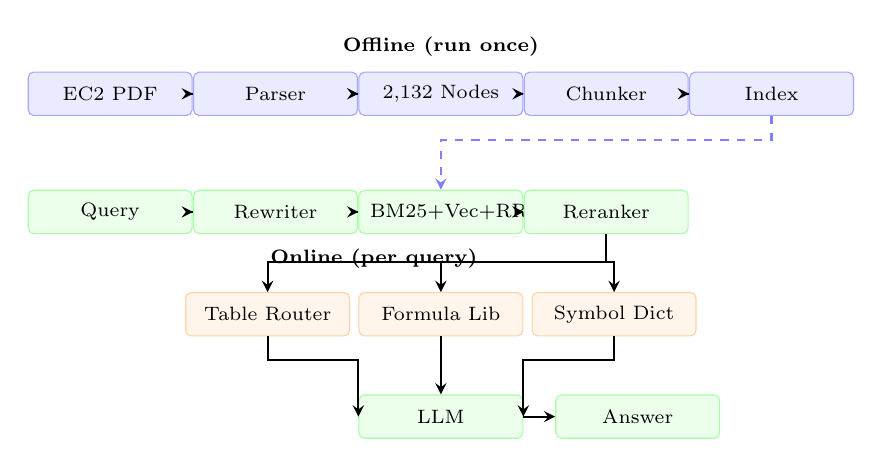
\begin{tikzpicture}[
  every node/.style={font=\scriptsize},
  box/.style={draw, rounded corners=2pt, inner sep=4pt,
              text width=1.8cm, align=center, minimum height=0.55cm},
  off/.style={box, fill=blue!8,   draw=blue!35},
  on/.style= {box, fill=green!8,  draw=green!35},
  en/.style= {box, fill=orange!8, draw=orange!35},
  arr/.style={-stealth, thick}
]

%% ---- OFFLINE ROW (y=0) ----------------------------------------
\node[off] (pdf)     at (0,   0)  {EC2 PDF};
\node[off] (parser)  at (2.1, 0)  {Parser};
\node[off] (nodes)   at (4.2, 0)  {2,132 Nodes};
\node[off] (chunker) at (6.3, 0)  {Chunker};
\node[off] (index)   at (8.4, 0)  {Index};

\draw[arr] (pdf)    -- (parser);
\draw[arr] (parser) -- (nodes);
\draw[arr] (nodes)  -- (chunker);
\draw[arr] (chunker)-- (index);

\node[font=\scriptsize\bfseries, above=2pt of pdf, xshift=4.2cm]
  {Offline (run once)};

%% ---- ONLINE ROW (y=-1.5) --------------------------------------
\node[on]  (query)   at (0,   -1.5) {Query};
\node[on]  (rewrite) at (2.1, -1.5) {Rewriter};
\node[on]  (hybrid)  at (4.2, -1.5) {BM25+Vec+RRF};
\node[on]  (rerank)  at (6.3, -1.5) {Reranker};

\draw[arr] (query)   -- (rewrite);
\draw[arr] (rewrite) -- (hybrid);
\draw[arr] (hybrid)  -- (rerank);

%% index -> hybrid (dashed)
\draw[arr, dashed, blue!50]
  (index.south) -- ++(0,-0.3) -| (hybrid.north);

%% ---- ENRICHMENT (y=-2.8) ---------------------------------------
\node[en] (tbl) at (2.0, -2.8) {Table Router};
\node[en] (fml) at (4.2, -2.8) {Formula Lib};
\node[en] (sym) at (6.4, -2.8) {Symbol Dict};

\draw[arr] (rerank.south) -- ++(0,-0.35)
  node[coordinate] (mid) {}
  (mid) -| (tbl.north);
\draw[arr] (mid) -| (fml.north);
\draw[arr] (mid) -| (sym.north);

%% ---- LLM + ANSWER (y=-4.1) ------------------------------------
\node[on]  (llm)    at (4.2, -4.1) {LLM};
\node[on]  (answer) at (6.7, -4.1) {Answer};

\draw[arr] (tbl.south) -- ++(0,-0.3) -| (llm.west);
\draw[arr] (fml.south) -- (llm.north);
\draw[arr] (sym.south) -- ++(0,-0.3) -| (llm.east);
\draw[arr] (llm) -- (answer);

\node[font=\scriptsize\bfseries, below=2pt of query, xshift=3.35cm]
  {Online (per query)};

\end{tikzpicture}
\caption{StructRAG pipeline. \textit{Offline} (top): the EC2 PDF is
  parsed into 2{,}132 typed nodes, chunked into 467 hierarchy-aware
  chunks, and stored in a vector+BM25 index.
  \textit{Online} (bottom): each query is rewritten, retrieved via
  hybrid BM25+vector RRF (dashed arrow shows index feed), reranked
  by a cross-encoder (top-8), enriched by three domain-specific
  injectors, and passed to the LLM for generation.}
\label{fig:arch}
\end{figure}

\subsection{Structural Parsing}

The French Eurocode~2 PDF (NF~EN~1992-1-1:2004, 211~pages) is parsed
with PyMuPDF~\cite{pymupdf} using a font-metric heuristic calibrated by
manual inspection.
Table~\ref{tab:font} shows the heading-level mapping.

\begin{table}[htbp]
  \centering
  \caption{Font-metric to node-type mapping for NF~EN~1992-1-1:2004.}
  \label{tab:font}
  \begin{tabular}{@{}cclc@{}}
    \toprule
    Size (pt) & Bold & Node type  & Level \\
    \midrule
    12 & Yes & Section    & 0 \\
    11 & Yes & Clause     & 1 \\
    10 & Yes & Sub-clause & 2 \\
    10 & No  & Paragraph  & 3 \\
     9 & No  & Note       & 3 \\
    \bottomrule
  \end{tabular}
\end{table}

A state machine assembles multi-span headings, maintains a parent stack
to build ancestor paths, and extracts cross-references via regex.
Output: 2{,}132 nodes---12 sections, 86 clauses, 275 sub-clauses,
1{,}326 paragraphs, 266 notes, 167 image/table blocks---with 569
nodes carrying automatically extracted cross-references.

Five critical tables (safety factors, concrete properties, exposure
classes, structural classification, minimum cover) are extracted by
pdfplumber into markdown text and indexed as additional searchable
chunks.

\subsection{Hierarchy-Aware Chunking}

The hierarchical chunker assembles each clause with all its direct child
paragraphs and notes into one retrievable chunk, prefixed by the full
ancestor breadcrumb:

\begin{verbatim}
[EC2 > Section 4 > 4.4 > 4.4.1 > 4.4.1.2]
4.4.1.2  Enrobage minimal, cmin

(1)P  Un enrobage minimal doit etre assure
      afin de permettre la transmission sure
      des efforts d'adherence ...
NOTE  La valeur de cmin,dur est donnee
      dans le Tableau 4.4N.
\end{verbatim}

This keeps three things co-located: the clause heading, the body text
with its applicability conditions, and any NOTE that overrides a
recommended value.
Chunks exceeding 512 tokens split at paragraph boundaries with the
heading repeated on each continuation.
Result: 467 hierarchical chunks.

For ablation, a flat baseline of 315 sliding-window chunks (512-token
window, 64-token overlap) is built from the same document.
A parent-child collection stores 1{,}818 paragraph-level child chunks
backed by 313 parent clause chunks.

\subsection{Indexing}

Chunks are stored in ChromaDB~\cite{chroma2023} using
\texttt{all-MiniLM-L6-v2}~\cite{reimers2019sbert} (22M parameters,
384-dimensional) as the embedding model.
An in-memory BM25Okapi~\cite{robertson2009bm25} index is built lazily
with French Snowball stemming.

\subsection{Hybrid Retrieval with RRF}

Vector and BM25 searches each return $k_{\text{fetch}} = \max(2k, 10)$
candidates; results are merged by Reciprocal Rank Fusion:
\begin{equation}
  \mathrm{score}_{\mathrm{RRF}}(d)
    = \frac{1}{k_{\mathrm{RRF}} + r_v(d)}
    + \frac{1}{k_{\mathrm{RRF}} + r_b(d)}
  \label{eq:rrf}
\end{equation}
where $r_v$ and $r_b$ are 1-indexed vector and BM25 ranks,
$k_{\mathrm{RRF}} = 60$~\cite{cormack2009rrf}, and absent documents
receive rank $+\infty$.
As shown in~\eqref{eq:rrf}, the score is rank-only and requires no
score calibration between the two retrieval methods.

A query-expansion heuristic appends table-lookup keywords when exposure
class (XC1--XA3) or structural class (S1--S6) identifiers appear in
the query, improving BM25 recall on tabular content.

\subsection{Cross-Encoder Reranking}

The top-20 RRF candidates are reranked by
\texttt{cross-encoder/ms-marco-MiniLM-L-6-v2}~\cite{nogueira2019passage},
which scores each (query, chunk) pair jointly.
The top-8 chunks are passed to generation; the reranker falls back to
the original RRF order if unavailable.

\subsection{Domain-Specific Enrichment}

\textit{Table Router.}
Detects lookup queries for cover values, safety factors, or exposure
classes and injects the relevant pre-extracted table rows.
Covered tables: 2.1N, 3.1, 4.1, 4.3N, 4.4N.

\textit{Formula Library.}
EC2 formulas are rendered as images in the PDF and are not text-
extractable.
24 key formulas are hand-transcribed (mathematical notation, variable
definitions, applicability conditions) and injected via a three-layer
trigger: (1)~clause number in query; (2)~keyword fast-path over
$\sim$40 engineering terms; (3)~embedding similarity above cosine
threshold 0.46.
The remaining 143 of 167 image-rendered formulas are not covered.

\textit{Symbol Dictionary.}
A lexicon of EC2 symbols ($c_{\mathrm{nom}}$, $\gamma_c$,
$\varepsilon_{cu2}$, etc.) with definitions is injected when a symbol
appears in the query.

\subsection{Generation}

The system prompt enforces three rules: answer only from the provided
context, write every formula explicitly when present, and say so when
the context is insufficient rather than generating from memory.
Primary backend: \texttt{openai/gpt-oss-120b} via Groq (131K context,
temperature 0.01).
A multi-backend interface supports NVIDIA build and Gemini APIs for the
four-model comparison.

A domain classifier (keyword scan over 80+ EC2 terms, plus a hard-block
list for clearly off-topic patterns) rejects non-engineering queries
before retrieval.

\subsection{Query Rewriting}

Before retrieval, a lightweight LLM (\texttt{openai/gpt-oss-20b} on
Groq) expands the query with EC2 terminology and clause identifiers to
improve both vector and BM25 recall.

% ── 4. Experimental Setup ────────────────────────────────────
\section{Experimental Setup}
\label{sec:setup}

\subsection{Corpus}

The indexed corpus is NF~EN~1992-1-1:2004 (French AFNOR edition of
Eurocode~2, 211~pages, born-digital PDF).
No other standard is indexed; ACI~318 and companion Eurocodes remain
future work.

\subsection{QA Benchmark}

The benchmark comprises 49 questions (50 constructed, 1 duplicate
removed) across eight categories: \textit{cover}~(12),
\textit{materials}~(8), \textit{design basis}~(1),
\textit{structural analysis}~(2), \textit{ultimate limit states}~(3),
\textit{serviceability}~(2), \textit{detailing}~(7),
\textit{cross-clause}~(2), and \textit{out-of-scope}~(5).
40 questions are in French (the document language); 9 are in English.
Questions, ground-truth answers, and ground-truth clause lists were
authored by the three student developers without external annotation.
No inter-annotator agreement statistic is available.

\subsection{Evaluation Metrics}

\textit{RAGAS metrics}~\cite{es2023ragas}.
Four LLM-as-judge metrics: faithfulness (claims grounded in context),
answer relevancy (answer addresses the question), context precision
(retrieved chunks are relevant), context recall (context contains the
ground truth).
Judge model: \texttt{openai/gpt-oss-120b} on Groq (same model as the
primary generation model; self-preference bias is uncontrolled).

\textit{Deterministic hallucination check.}
Each answer is scanned for clause-number patterns
(e.g.\ \texttt{4.4.1.2}, \texttt{6.2.2}).
Any cited clause not present among the 2{,}132 parsed nodes is
flagged as a hallucinated citation.
This check is independent of any LLM judge.

\textit{Refusal rate.}
Fraction of the 5 out-of-scope questions correctly rejected before
reaching the LLM.

\subsection{Models Evaluated}

Four models are compared under identical retrieval and prompt
configuration at temperature 0.01:
\begin{enumerate}
  \item \texttt{openai/gpt-oss-120b} via Groq (131K context)
  \item \texttt{nvidia/llama-3.3-nemotron-super-49b-v1} via NVIDIA
  \item \texttt{meta/llama-3.1-70b-instruct} via NVIDIA
  \item \texttt{z-ai/glm-5.2} via NVIDIA (1M context)
\end{enumerate}

% ── 5. Evaluation Results ────────────────────────────────────
\section{Evaluation Results}
\label{sec:eval}

\subsection{RAGAS Benchmark}

Two scoring runs exist in our data.
\textit{Run~A} passed answers to the faithfulness judge without
providing the retrieved context passages; the judge could only check
whether the answer sounded consistent with itself.
\textit{Run~B} passed both the answer and the retrieved context.
Run~A produced faithfulness of 0.97 for \texttt{gpt-oss-120b}; Run~B
produced 0.32 for the same answers.

Run~A faithfulness is not a valid measure: a judge that never sees the
context cannot assess whether claims are grounded in it.
We therefore report Run~B faithfulness where available and mark
Run~A faithfulness as invalid.
Table~\ref{tab:ragas} shows the results.

% [RESCORE]: before submission, run one pinned context-aware judge
% for all 4 models and replace the --- cells and the A* values.
% The 0.97 / 0.95 / 0.99 cells marked A* must not appear in the
% final version — they are not measuring faithfulness correctly.

\begin{table}[htbp]
  \centering
  \caption{RAGAS benchmark (44 in-scope questions).
    Run~A: judge saw answer only, not context --- invalid for
    faithfulness.
    Run~B: judge saw answer and context --- valid.
    Cells marked ${}^*$ are Run~A values pending a valid re-score.
    % [RESCORE]: replace all ${}^*$ cells and fill --- before submission.
  }
  \label{tab:ragas}
  \resizebox{\linewidth}{!}{%
  \begin{tabular}{@{}lcccc@{}}
    \toprule
    Model & Faith. & Ans.\ Rel. & Ctx.\ Prec. & Ctx.\ Rec. \\
    \midrule
    \texttt{gpt-oss-120b}
      & 0.32 & 0.77 & 0.69 & 0.27 \\
    \texttt{nemotron-49b}
      & $0.95^*$ & 0.67 & --- & --- \\
    \texttt{llama-3.1-70b}
      & $0.99^*$ & 0.68 & --- & --- \\
    \texttt{glm-5.2}
      & 0.68 & 0.64 & 0.68 & 0.63 \\
    \bottomrule
  \end{tabular}}
  \\[4pt]
  \small
  Note: context recall of 0.27 for \texttt{gpt-oss-120b} means the
  pipeline retrieves roughly one quarter of the ground-truth
  information per question on average.
  This is the most operationally significant result in this table
  and the primary target for future retrieval improvements.
\end{table}

\subsection{Hallucination and Out-of-Scope Refusal}

Table~\ref{tab:hallucination} reports the deterministic hallucination
check and classifier refusal results.

\begin{table}[htbp]
  \centering
  \caption{Hallucination (44 in-scope questions) and refusal
    (5 out-of-scope questions) results.}
  \label{tab:hallucination}
  \begin{tabular}{@{}lcc@{}}
    \toprule
    Model & Halluc.\ Rate & Refusal Rate \\
    \midrule
    \texttt{gpt-oss-120b}  & 0\% (0/44)  & 100\% (5/5) \\
    \texttt{nemotron-49b}  & 0\% (0/44)  & 100\% (5/5) \\
    \texttt{llama-3.1-70b} & 2\% (1/44)  & 100\% (5/5) \\
    \texttt{glm-5.2}       & 0\% (0/44)  &  40\% (2/5) \\
    \bottomrule
  \end{tabular}
\end{table}

\noindent
Three of four models produced zero hallucinated clause citations.
\texttt{llama-3.1-70b} produced one instance.
The 100\% refusal rate for three models reflects complete rejection of
all five out-of-scope queries (wind load per EN~1991, seismic behavior
factor per EN~1998, water-cement ratio per EN~206-1).
\texttt{glm-5.2}'s 40\% refusal rate means it passed three borderline
queries through the classifier; this contributes to its higher context
recall.

\subsection{Retrieval Ablation}

Table~\ref{tab:ablation} traces cumulative improvements on the
14-question evaluation harness used during development.
Scores are human-judged correctness by the system developers.

\begin{table}[htbp]
  \centering
  \caption{Retrieval ablation (14-question subset; human-judged
    correct / 14). Note: v3 changes two variables simultaneously
    (reranker and parent-child chunking); the individual contributions
    cannot be separated from this data.}
  \label{tab:ablation}
  \begin{tabular}{@{}lp{4.6cm}c@{}}
    \toprule
    Run & Changes & Score \\
    \midrule
    v1 & $k{=}5$, vector only, no tables    & 3/14 \\
    v2 & $k{=}8$, BM25+vector RRF, tables   & 7/14 \\
    v3 & v2 + reranker + parent-child chunks & 9/14 \\
    \bottomrule
  \end{tabular}
\end{table}

\noindent
The full flat-baseline pipeline (315 sliding-window chunks, no
structural metadata) was not run through the 49-question RAGAS
benchmark; only the hierarchical pipeline was scored end-to-end.
A direct hierarchical-vs-flat comparison on the full benchmark is the
most important missing experiment for validating the central claim of
the paper.

% ── 6. Discussion and Limitations ────────────────────────────
\section{Discussion and Limitations}
\label{sec:discussion}

\textit{Context recall is the primary operational problem.}
Context recall of 0.27 for \texttt{gpt-oss-120b} means the retriever
delivers, on average, only about one quarter of the ground-truth
information needed to answer a question.
High faithfulness and answer relevancy are secondary if the context
itself is incomplete.
The two most likely causes are: (a)~the 143 image-rendered formulas
that are entirely absent from the index; (b)~cross-reference questions
that require information spread across multiple clauses.

\textit{Faithfulness judge validity.}
Run~A faithfulness (0.95--0.99) was computed by a judge that never saw
the retrieved passages.
Such a judge measures surface plausibility, not grounding.
Run~B (faithfulness 0.32 for \texttt{gpt-oss-120b}) is the correct
measurement, and its lower value is expected: it catches cases where
the model extends or reframes the context rather than quoting it
directly.
The 0.32 value should be interpreted as ``answers do not directly
copy-quote the context'' rather than as evidence of hallucination.

\textit{Judge self-preference bias.}
\texttt{gpt-oss-120b} is both a system under test and the RAGAS judge.
LLM-as-judge setups are known to exhibit self-preference
bias~\cite{es2023ragas}; our setup does not control for this.
An independent judge model is required for a publishable comparison.

\textit{Missing flat-baseline comparison.}
The 315-chunk flat baseline was built and indexed, and is exercised by
the v1 ablation row, but was never evaluated end-to-end on the full
49-question benchmark.
Without this comparison, the claim that hierarchical chunking
outperforms flat chunking rests on a 14-question human-judged pilot
rather than the full RAGAS evaluation.
Running the flat baseline through the complete benchmark is the
single highest-priority experiment for a revised submission.

\textit{Ablation confound.}
Run v3 changes two independent variables simultaneously: the cross-
encoder reranker and the switch from hierarchical to parent-child
chunks.
The 7/14$\to$9/14 improvement cannot be attributed to either component
individually from the current data.

\textit{Annotation by the developers.}
All 49 benchmark questions, ground-truth answers, and clause
annotations were authored by the three system developers without
external validators.
No inter-annotator agreement statistic is reported.
This is a standard limitation for pilot systems of this size and
should be stated explicitly.

\textit{Formula coverage gap.}
EC2 has 167 image-rendered formula blocks.
24 are hand-transcribed; the remaining 143 are not text-retrievable.
This is the largest single cause of missed ground-truth information.

\textit{Corpus scope.}
Only NF~EN~1992-1-1:2004 is indexed.
Questions referencing EN~206-1, EN~1990, or EN~1998 are correctly
refused but cannot be answered.
The paper's framing as a system for ``civil engineering standards''
exceeds the scope of what is actually demonstrated.

% ── 7. Conclusion ─────────────────────────────────────────────
\section{Conclusion}
\label{sec:conclusion}

We presented StructRAG, a RAG system for Eurocode~2 that maps the
document's own clause hierarchy onto the indexing unit.
A font-metric parser, breadcrumb-prefixed clause chunking, hybrid
BM25+vector RRF retrieval, cross-encoder reranking, and domain-specific
table and formula injectors raise the correct-answer rate from 3/14 to
9/14 on a 14-question development set.
A deterministic hallucination check verifies cited clause numbers
against the 2{,}132 parsed nodes; three of four evaluated models
produce zero hallucinated citations on 44 in-scope questions.

The evaluation has two open issues that must be resolved before
submission to a peer-reviewed venue: (1)~a context-aware, single-run
RAGAS re-score using an independent judge model; and (2)~an end-to-end
comparison of the hierarchical pipeline against the flat baseline on
the full 49-question benchmark.
Both experiments are executable with the existing codebase and data.

Once those results are in hand, this work provides a concrete and
reproducible demonstration that clause-boundary chunking with ancestor
breadcrumbs meaningfully improves retrieval quality on a safety-critical
normative corpus, without requiring LLM fine-tuning.

% ── Bibliography ──────────────────────────────────────────────
\bibliographystyle{IEEEtran}
\bibliography{references}

\end{document}
